
% This thesis template is based on the report class of
% latex. Yout do not need to change this.
\documentclass[12pt, a4paper]{report}

% This template uses the babel package for customizing
% labels like Figure/Abbildung etc. Please adust the
% language parameter if necessary. Currently, it is
% set to 'english'. If you write in German adjust the
% parameter to 'ngerman'
\usepackage[english]{babel}

% This includes all variables that are used in this work
% Use this document to specify your name, your reviewers
% and other values that you would like to maintain
% in one place.
\newcommand\myname{Gunharth Randolf}
\newcommand\mypkz{1810738273}

\newcommand\myfirstreviewer{Prof. (FH) Dr. Michael Kohlegger}
\newcommand\mysecondreviewer{Lukas Demetz, PhD}

\newcommand\mytitle{From Native to Progressive Web App \\ A Proof of Concept}

% The value below is the date that you finished your work. This
% date appears on you work's cover page and in the "Eidesstattliche
% Erklärung".
\newcommand\mydate{29. July 2019}

% This template assumes that you are studying Data Science &
% Intelligent Analytics. Please Change if necessary
\newcommand\academictitle{}
\newcommand\worktype{}
\newcommand\studyprogram{Web Communication \& Information Systems}


% This includes all packages and presets. You do not need
% to change this file unless you want to add new packages
% or change the presets of one of the used packages.
%\usepackage{bookman}  % Font package
%\usepackage[light]{CrimsonPro}
\usepackage{pxfonts}
\usepackage[T1]{fontenc}
\usepackage{graphicx}
\usepackage[utf8]{inputenc}
\usepackage{blindtext}  % Used for dummy text segments
\usepackage{natbib}
\usepackage{hyperref}
\usepackage{booktabs}
\usepackage{xcolor}
\usepackage{listings}
\lstset{numberbychapter=false}
\iflanguage{english}{\renewcommand{\lstlistlistingname}{List of Listings}}{\renewcommand{\lstlistlistingname}{Listingsverzeichnis}}

\usepackage{fancyhdr}  % Head and footer styling
\fancyhead[RO]{\thepage}
\fancyhead[LO]{\nouppercase\leftmark}
\renewcommand\headrulewidth{0.5pt}
\renewcommand\footrulewidth{0pt}

\usepackage[a4paper, left=3.5cm, right=3cm, top=3.5cm, bottom=3cm]{geometry}
\setlength{\headheight}{15pt}

\usepackage[title, titletoc, header]{appendix}
\renewcommand{\appendixname}{Appendix}

\usepackage{titlesec}
\titleformat{\chapter}{\bf \LARGE}{\thechapter.}{16pt}{\LARGE}

\usepackage{chngcntr}
\counterwithout{figure}{chapter}
\counterwithout{table}{chapter}

\bibliographystyle{apalike}
\pagestyle{headings}
\setlength{\parindent}{0em}
\setlength{\parskip}{1.5em}
\renewcommand{\baselinestretch}{1.13}

\newcommand\frontmatter{
    \pagestyle{fancy}
    \fancyfoot{}
    \pagenumbering{Roman}
}

\newcommand\mainmatter{
    \pagenumbering{arabic}
}

\newcommand\backmatter{
    \pagenumbering{arabic}
    \renewcommand{\thepage}{A\arabic{page}}
}        

\lstset{
    numberstyle=\tiny,
    numbers=left,
    showstringspaces=false,
    breaklines=true,
    commentstyle=\itshape\color{darkgray},
    basicstyle=\ttfamily,
    stringstyle=\color{orange},
    keywordstyle=\bf\color{green!40!black},
    identifierstyle=\color{blue}
}

\hypersetup{
  pdftitle    = \mytitle,
  pdfsubject  = \worktype,
  pdfauthor   = \myname,
  pdfcreator  = {pdflatex using template provided by University of Applied Sciences FH Kufstein Tirol},
  bookmarksnumbered = true,
  colorlinks = true,
  linkcolor = blue,
  citecolor = green,
  urlcolor = orange
}


% This includes custom latex commands. You can use this
% file to create your own command sequences.
\newcommand{\fh}{\textsc{FH Kufstein Tirol}}

\newcommand{\fig}[4]{
    \begin{figure}[ht]
        \centering
        \includegraphics[width=#4\textwidth]{#1}
        \caption{#2}
        \label{#3}
    \end{figure}
}


% If you want to print your thesis in black and white
% uncomment the following section

% \hypersetup{
%     colorlinks=false,
%     pdfborder = 0 0 0
% }
% \lstset{
%     commentstyle=\itshape,
%     basicstyle=\ttfamily,
%     stringstyle=\color{black},
%     keywordstyle=\bf,
%     identifierstyle=\color{black}
% }

\begin{document}

    \frontmatter

    % This places the front matter. You do not need to
    % change this file. All thesis-specific values are
    % imported from ``core/variables.tex``.
    \begin{titlepage}

    \vfill
    \begin{center}
      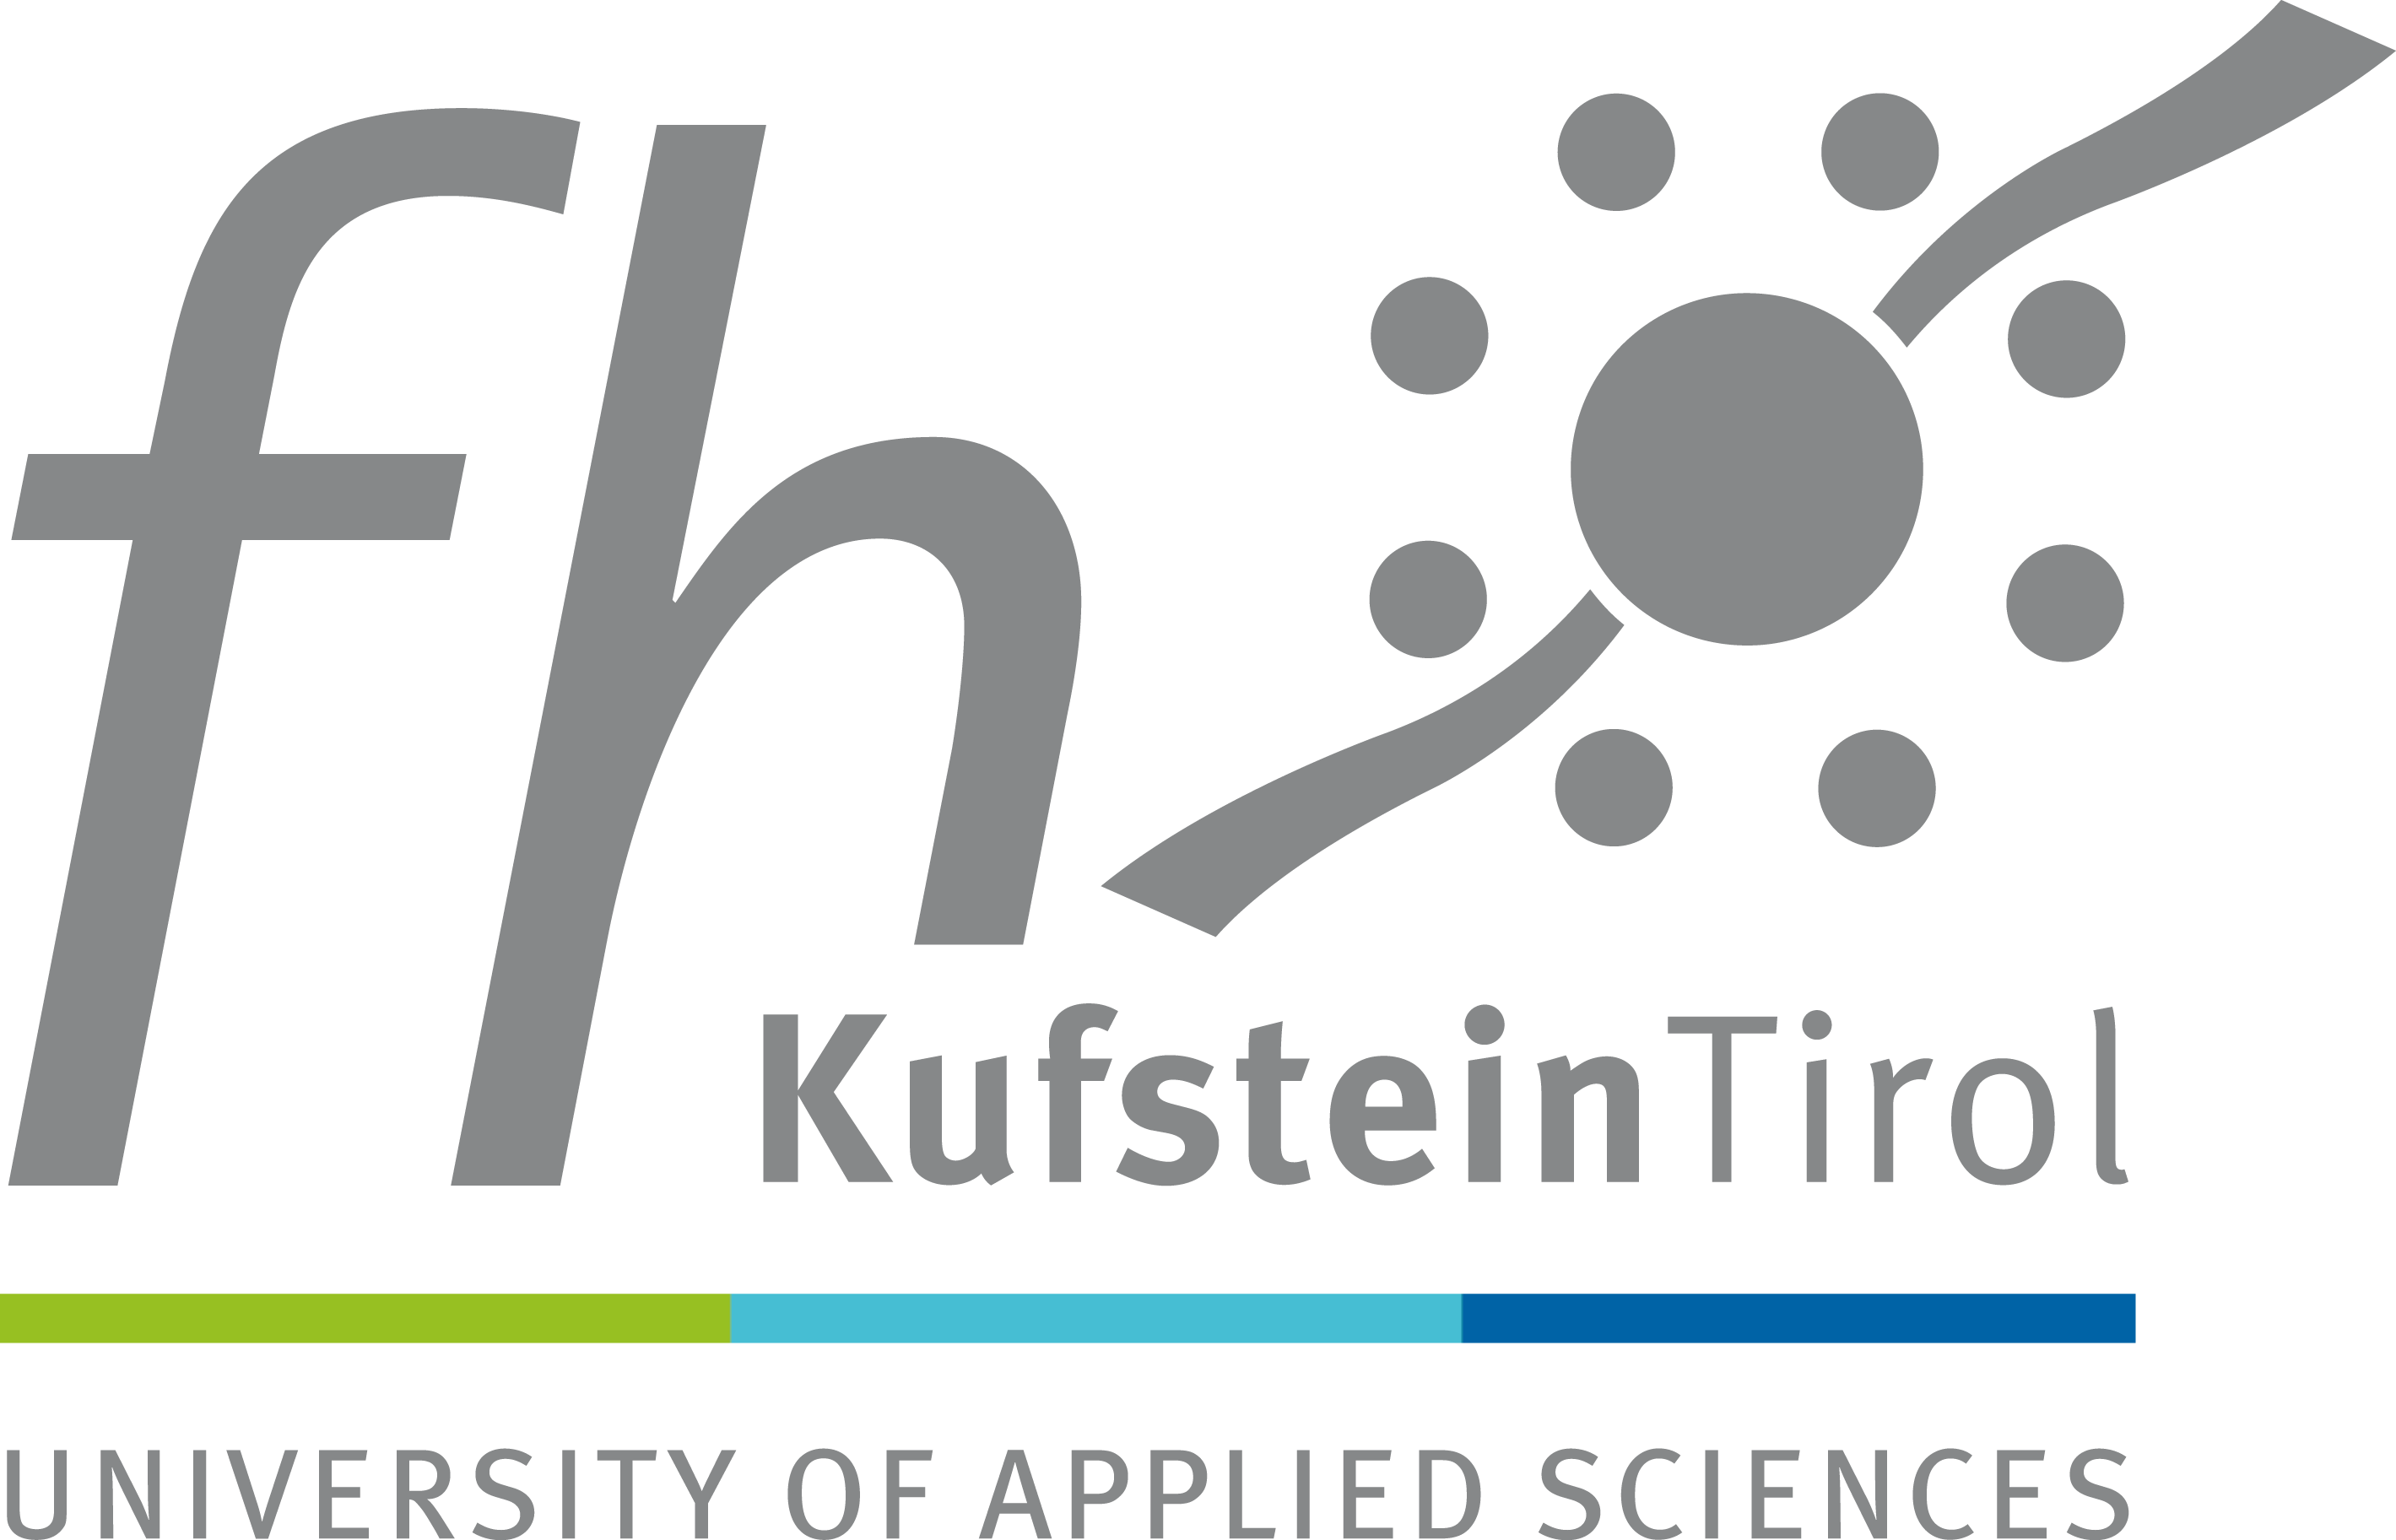
\includegraphics[width=4.5cm]{img/kufstein_logo.png} \\
    \end{center}
    \vfill

    \begin{center}
      \Large \textbf{\mytitle}
    \end{center}
    \vfill

    % \begin{center}
    %   %\condMASTER{\Large Masterarbeit}{\Large Bachelorarbeit}
    %   \worktype
    % \end{center}
    % \vfill

    % \begin{center}
    %  zur Erlangung des akademischen Grades\\
    %  \large \textbf{\academictitle}
    % \end{center}
    % \vfill

    \begin{center}
      % As part of the lecture:\\
      \textbf{\myname}\\
      \vspace{0.1cm}
      \textbf{\mypkz}\\
      \vspace{0.1cm}
      \textbf{Entwicklung \& Betrieb Mobiler Informationssysteme}\\
      \vspace{0.1cm}
      \textbf{\studyprogram}\\
      \vspace{0.1cm}
      \textbf{\mydate}
    \end{center}
    \vfill
  \end{titlepage}


    % This places the "Eidesstattliche Erklärung". This
    % Document is always in German, even if your work is
    % written in English.
    % \chapter*{Eidesstattliche Erklärung}
\thispagestyle{empty}

Ich erkläre hiermit, dass ich die vorliegende Masterarbeit selbständig und ohne fremde Hilfsmittel verfasst und in der Bearbeitung und Abfassung keine anderen als die angegebenen Quellen oder Hilfsmittel benutzt sowie wörtliche und sinngemäße Zitate als solche gekennzeichnet habe. Die vorliegende Masterarbeit wurde nicht anderweitig für Prüfungszwecke vorgelegt.

\vspace{2cm}
Kufstein, \mydate

\vspace{2cm}
\rule{10cm}{1pt}\\
\myname{}



    % This will include a "Sperrvermerk". This document
    % is always in German, even if your work is written
    % in English. Please remove this line, if necessary.
    % \chapter*{Sperrvermerk}
\thispagestyle{empty}

Ich habe die Sperrung meiner Masterarbeit beantragt, welche von der Studiengangsleitung genehmigt wurde.

\vspace{2cm}
Kufstein, \mydate

\vspace{2cm}
\rule{10cm}{1pt}\\
\myname{}


        % This adds a german and an english summary to your work.
        % You always have to add both, independent of whether your
        % work is done in german or english
        % \thispagestyle{empty}

\textbf{FH Kufstein Tirol\\Data Science \& Intelligent Analytics}

Abstract of the thesis: \textbf{\mytitle}

\textbf{Author:} \myname\\
\textbf{First reviewer:} \myfirstreviewer\\
\textbf{Second reviewer:} \mysecondreviewer\\

% Your text goes here (aprox. 350 words)
\Blindtext[2][1]

% End with date
\mydate{}

        % \thispagestyle{empty}

\textbf{FH Kufstein Tirol\\Data Science \& Intelligent Analytics}

{Kurzfassung der Masterarbeit: \textbf{\mytitle}}

\textbf{Verfasser:} \myname\\
\textbf{Erstgutachter:} \myfirstreviewer\\
\textbf{Zweitgutachter:} \mysecondreviewer\\

% Your text goes here (aprox. 350 words)
\Blindtext[2][1]

% End with date
\mydate{}


        \thispagestyle{empty}

\textbf{Abstract}

Lorem ipsum


    % This inserts all necessary tables into your work.
    \tableofcontents
    % \listoffigures
    % \listoftables

    % Use this if you have any code listings
    % \lstlistoflistings

    \mainmatter

    % This places the actual chapters. The files referenced here
    % are just an example. You can add additional chapters if
    % necessary
    % \chapter{Introduction}

\blindtext \citet{Shearer2000}

\section{Problem Situation}

\blindtext

\fig{img/sax_approximated_series}{Sax approximation of a time series}{fig:sax}{0.5}

As can be seen in Figure~\ref{fig:sax} \ldots

\section{Objectives}

\blindtext

\section{Methods}

\blindtext

\section{Structure}

\blindtext

\section{Tables}

Table~\ref{tab:table-one} shows an example table.

\begin{table}[htbp]
    \centering
    \caption{This is a table}
    \label{tab:table-one}
    \begin{tabular}{lll}
        \addlinespace
        \toprule
        Column 1 & Column 2 & Column 3 \\
        \midrule
        A     & B     & C \\
        D     & E     & F \\
        G     & H     & I \\
        \bottomrule
    \end{tabular}
\end{table}

\section{Source Code}

\begin{lstlisting}[language=Java, caption=Hello World in Java, label=lst:hello-world-java]
public class Hello {
    public static void main(String[] args) {
        System.out.println("Hello World");
    }
}
\end{lstlisting}

Listing~\ref{lst:hello-world-java} shows the classic Hello World in Java.

\lstinputlisting[language=Python, caption=Hello World in JavaScript, label=lst:hello-world-py]{./lst/hello.py}

Listing~\ref{lst:hello-world-py} shows the classic Hello World in Python.

    % \chapter{Foundations}

\blindtext[1]

\section{Machine Learning}

\Blindtext[4][1]

\section{Deep Learning}

\Blindtext[4][1]

    % \chapter{Study Design}

\Blindtext[4][1]

    % \chapter{Results}

\Blindtext[4][1]

    % \chapter{Discussion}

\Blindtext[4][1]

    \chapter{Introduction}

In 2015 the Google Developer Alex Russel first drafted the term Progressive Web Apps (PWAs) and formulated the concept of PWAs as it stands today.

Full Progressive App support will distinguish engaging, immersive experiences on the web from the “legacy web”. Progressive App design offers us a way to build better experiences across devices and contexts within a single codebase but it’s going to require a deep shift in our understanding and tools. \citep{russellProgressiveWebApps2015}

Since then, notably Google and its Chrome browser focus on the implementation of all necessary technologies in order to fully support PWAs. Nearly every new release offers the Chrome browser adds further support for PWAs. As an example, at the time of writing Chrome 76 shows an install icon to the left of the address bar, if a site meets the Progressive Web App installability criteria\footnote{\url{https://developers.google.com/web/fundamentals/app-install-banners\#criteria}}.

So far, the bedrock for engaging and immersive experiences on mobile devices has been bound to the development of native and/or hybrid apps. However, developing a native application is an expensive solution. Programmers spend years learning to code heavy native apps and app owners usually invest a huge budget finding a development team \citep{nguyen2019progressive}. That said, at least two versions need to be developed, maintained and published to the Apple and Google App Stores respectively.

As PWAs are still a rather new concept there are known limitations in terms of unified browser support of APIs\footnote{\url{https://whatwebcando.today}}, missing filesystem access and platform-level features integrations like calendar and contacts \citep{biorn-hansenProgressiveWebApps2018,malavoltaNativeAppsWeb2016}. However, there are many applications that do not depend on the before mentioned limitations. On 15th July 2019 Twitter announced its new website, which is a PWA build on one code base feeding all devices and browsers that are accessing the site on the Web. The goal for the new site was to make it easier and faster to develop new features for people worldwide and to provide each person and each device with the right experience \citep{croomBuildingNewTwitter2019}.

The purpose for this study is to look at the technical side of PWAs, whereby the following questions will be answered. First, whether it is possible to take an existing mobile app as a prototype and re-build the app as a PWA. Second, what services and programming languages are best fitted in doing so and how well do they support the development of a PWA? Finally, I discuss my findings and any limitations I might have encountered.

    % \chapter{Background}

What backgrounds?

    % \chapter{Related Work}

Related work?

    \chapter{Methods}

This study implements three research methods to gain a broader understanding of the possibilities, state of research and technological practices regarding Progressive Web Apps.

\section{Literature Search}

Our searches for academic involvement in Progressive Web Apps returned a very limited amount of results as per July 2017 \citep{biorn-hansenProgressiveWebApps2018}. The same search performed 2 years later doesn't reveal any further major releases on this topic. Scientific research is still pretty sparse. However, technology related publishers have picked up the topic with a handful of publications in 2017 and 2018 \citep{humeProgressiveWebApps2018,aterBuildingProgressiveWeb2017}. In 2019 though, there seems to be only one notable publication; a practical guide to PWAs by Liebel written in the German language \citep{liebelProgressiveWebApps2019}.

Interestingly, I was not able to find any scientific research on the commercial aspects of PWA. A comparison on budgets and running costs required by native/hybrid apps versus a PWA. Further st

\section{Related Works}
The Google Web Fundamentals group acts as the driving force behind the documentation on PWA related topics and the creation of blog posts and tutorials. As the supporting technologies advance with every Chrome browser release, the Web Fundamentals website\footnote{\url{https://developers.google.com/web/fundamentals}} is the foundation for upcoming research and studies.

Other than Google-created content, online platforms such as Medium blog posts\footnote{\url{https://medium.com/search?q=Progressive\%20Web\%20Apps}} and Youtube tutorials\footnote{\url{https://www.youtube.com/results?search_query=Progressive+Web+Apps}} lay the foundation of technical research for this study. Notably, the technical series of articles about PWA published by Eder Ramírez Hernández\footnote{\url{https://medium.com/@eder.ramirez87}} on Medium were extremely informative.

\section{Technical Implementation}
To gain a better understanding of the possibilities of Progressive Web Apps a PWA was developed. The motivation for the PWA was to take an existing native application as a reference and to re-create the application as a Progressive Web App. For this purpose I picked the \textit{Beer With Me}\footnote{\url{https://beerwithme.se/}} application, which is available on the Apple App Store as well as on Google Play. As stated by the Swedish developers Antonsson, Knutsson and Tidbeck "Beer With Me is a social application to notify your friends when you are drinking so that they can join".

    \chapter{Concepts \& Technical Implementation}
This chapter provides a detailed look at the required concepts and the technical implementation of the PWA. The project has been open-sourced to allow verification of the results\footnote{\url{https://github.com/gunharth/bwm}}. Further, the application is available online\footnote{\url{https://bwm.gunicode.com}}.

\section{Requirements}

The following section outlines the concepts and requirements used for the project by looking at the core functionality of the original \textit{Beer with Me} app.

\textbf{Progressive Web App}. The functional clone of the \textit{Beer with Me} app must implement all relevant techniques as outlined by the Progressive Web App specifications. Technologies include Service Workers, Application Shell (AppShell), Web App Manifest and serving the demo installation over HTTPS. Further, it is the intention to follow the 10 principal concepts, which lay the foundation for Progressive Web Applications, as closely as possible: Progressive, Responsive, Installable, Connectivity Independent, App-Like, Fresh, Safe, Discoverable, Re-engageable and Linkable \citep{osmaniGettingStartedProgressive2015}.

\textbf{Authentication and Authorization}. Users must be able to register for the service with a combination of E-Mail and Password. As an alternative an existing Google account may be used in order to login directly.

\textbf{Realtime Database}. Data is stored in a cloud-hosted database and synchronized in realtime to every connected client.

\textbf{Realtime Notifications}. If enabled by the user push-notifications shall be send to the user in realtime, whenever a new user registers for the service or when a new post was published by a user.

\textbf{Realtime Map}. If enabled by the user his/her current geolocation is saved and displayed on an online map.

\textbf{Single Page App (SPA)}. The app shall be implemented as a Single Page App with one of the main JavaScript frameworks (React, Angular or Vue.js).

Option to add a photo using the device’s camera


Frontend, Backend framework/system
straight forward deployment process

The following topics were defined as being not part of the requirements, as they do not have an impact on the used technologies of the PWA, nor do they have an effect on the results of this study. Hence, design considerations of the application can be neglected, nor is the intention to copy the interface and design of the original \textit{Beer with Me} app. The resulting PWA focusses on the implementation of the functionality and not on offering a identical clone of the original. Further, all functions are implemented as a proof-of-concept following the MVP spirit \citep{wikipediaMinimumViableProduct2019}. Thus, to make it a user centric production ready PWA further development cycles are required.


\section{Technical Implementation of Requirements}
As per the actual implementation of the PWA the goal was to base the solution on the least different providers on the one hand, as well as a minimum in terms of coding and programming languages. Hence, the front-end of the application uses the basic building blocks of regular web sites being HTML, CSS and JavaScript in form of the JavaScript framework Vue.js. To satisfy the back-end Firebase was picked as the sole solution provider.

\subsection{Single Page App (SPA) \& Progressive Web App}
For the development of the frontend the JavaScript framework Vue.js\footnote{\url{https://vuejs.org}} and its ecosystem was used. The Vue Cli\footnote{\url{https://cli.vuejs.org}} offers great tooling support for Vue.js developments - among other features it comes with a preset for installing a Progressive Web App skeleton.

\begin{lstlisting}[language=bash, caption=Installation and project creation commands with the Vue Cli, label=lst:vue-cli]
  $ npm install -g @vue/cli
  $ vue create beerwithme
\end{lstlisting}

On project creation Vue Cli offers you to manually select the features that will be installed. Next to Progressive Web Application support the Vue Router and Vuex was installed. The Router enables navigation services within a SPA and Vuex is responsible for the management of state within the application.

\fig{img/vue_project_creation}{Installation options for a Vue.js project}{fig:vue-project-creation}{1}

The Vue Cli PWA support comes with Workbox\footnote{\url{https://developers.google.com/web/tools/workbox}} installed - a library developed by Google for adding offline support to web applications. Among other features it mainly helps with the automatic creation and management of application pre-cache and the App Shell .

\begin{lstlisting}[language=JavaScript, caption=Service Worker with Workbox and Firebase specific initiation (firebase-messaging-sw.js), label=lst:serviceworker]
  importScripts("https://www.gstatic.com/firebasejs/5.6.0/firebase-app.js");
  importScripts("https://www.gstatic.com/firebasejs/5.6.0/firebase-messaging.js");

  self.__precacheManifest = [].concat(self.__precacheManifest || []);
  workbox.precaching.suppressWarnings();
  workbox.precaching.precacheAndRoute(self.__precacheManifest, {});

  workbox.routing.registerRoute(
    new RegExp(
      "https://firebasestorage.googleapis.com/v0/b/bmwgunicode.appspot.com/.*"
    ),
    workbox.strategies.staleWhileRevalidate()
  );

  firebase.initializeApp({
    messagingSenderId: "ID"
  });

\end{lstlisting}

For the front-end design of the app Vuetify\footnote{\url{https://vuetifyjs.com}} was used. Vuetify is a responsive design component framework for Vue.js based on the material design\footnote{\url{https://material.io}} guidelines developed by Google.

\begin{lstlisting}[language=bash, caption=Command to add Vuetify to the Vue.js project, label=lst:vuetify]
  $ vue add vuetify
\end{lstlisting}

The map functionality was implemented by using the npm package vue2-leaflet\footnote{\url{https://www.npmjs.com/package/vue2-leaflet}}, which is a Vue wrapper library for the open-source JavaScript library Leaflet\footnote{\url{https://leafletjs.com}}. Map tiles are served from OpenStreetMap\footnote{\url{https://www.openstreetmap.org}}.
\\

\begin{figure}
  \centering
  \begin{subfigure}{.5\textwidth}
    \centering
    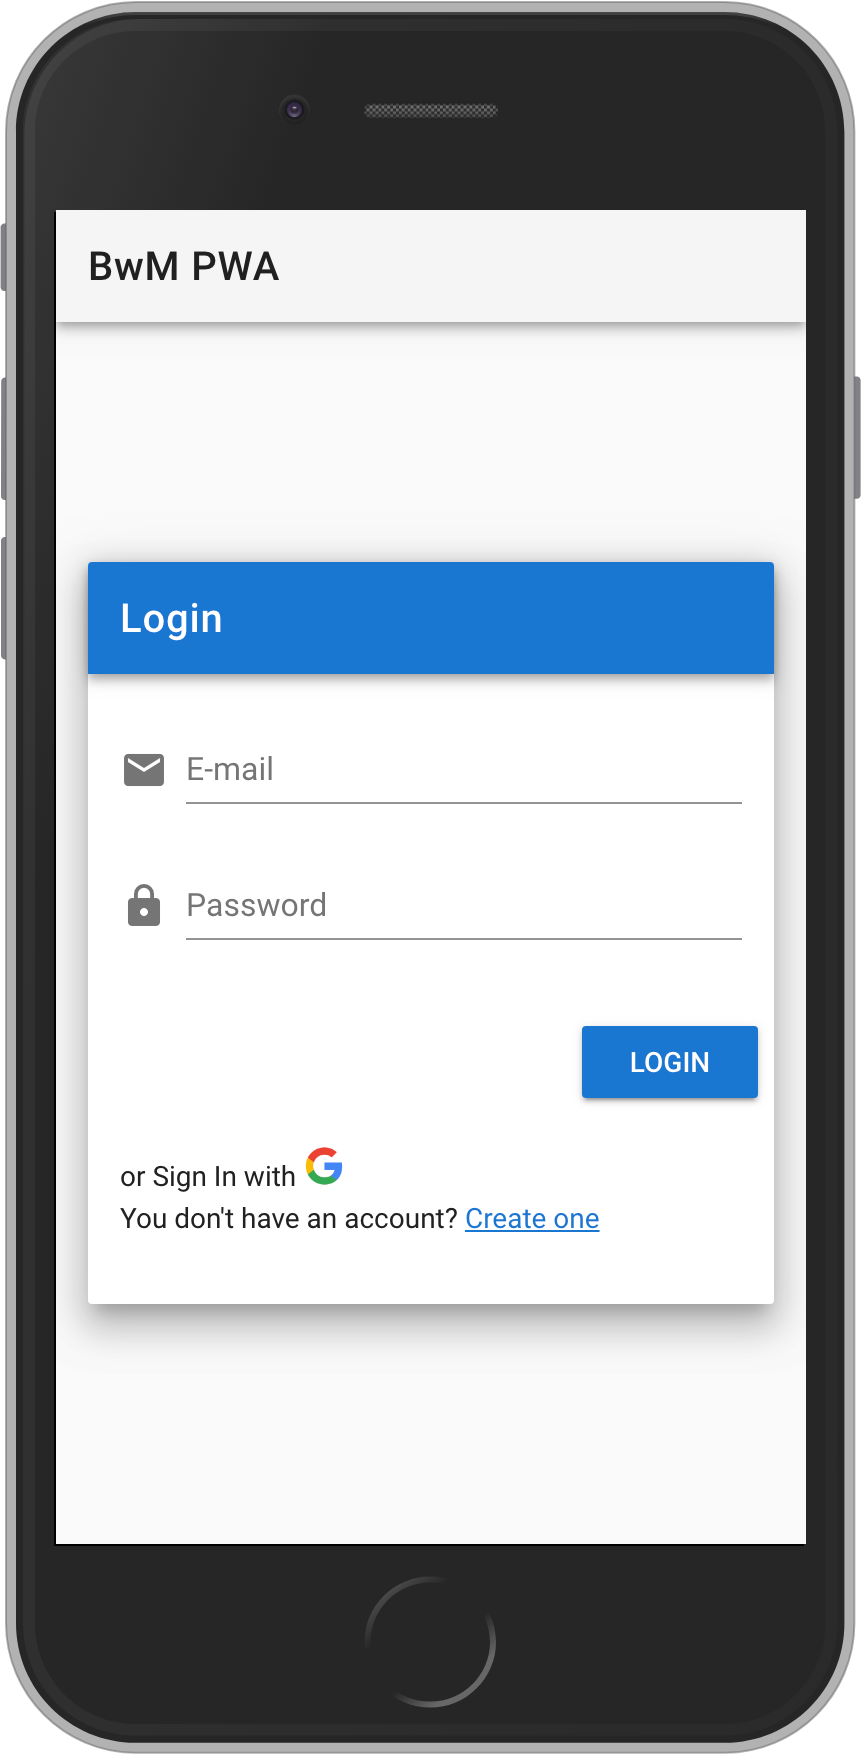
\includegraphics[width=.7\linewidth]{img/screen01}
    \caption{Login screen}
    \label{fig:sub1}
  \end{subfigure}%
  \begin{subfigure}{.5\textwidth}
    \centering
    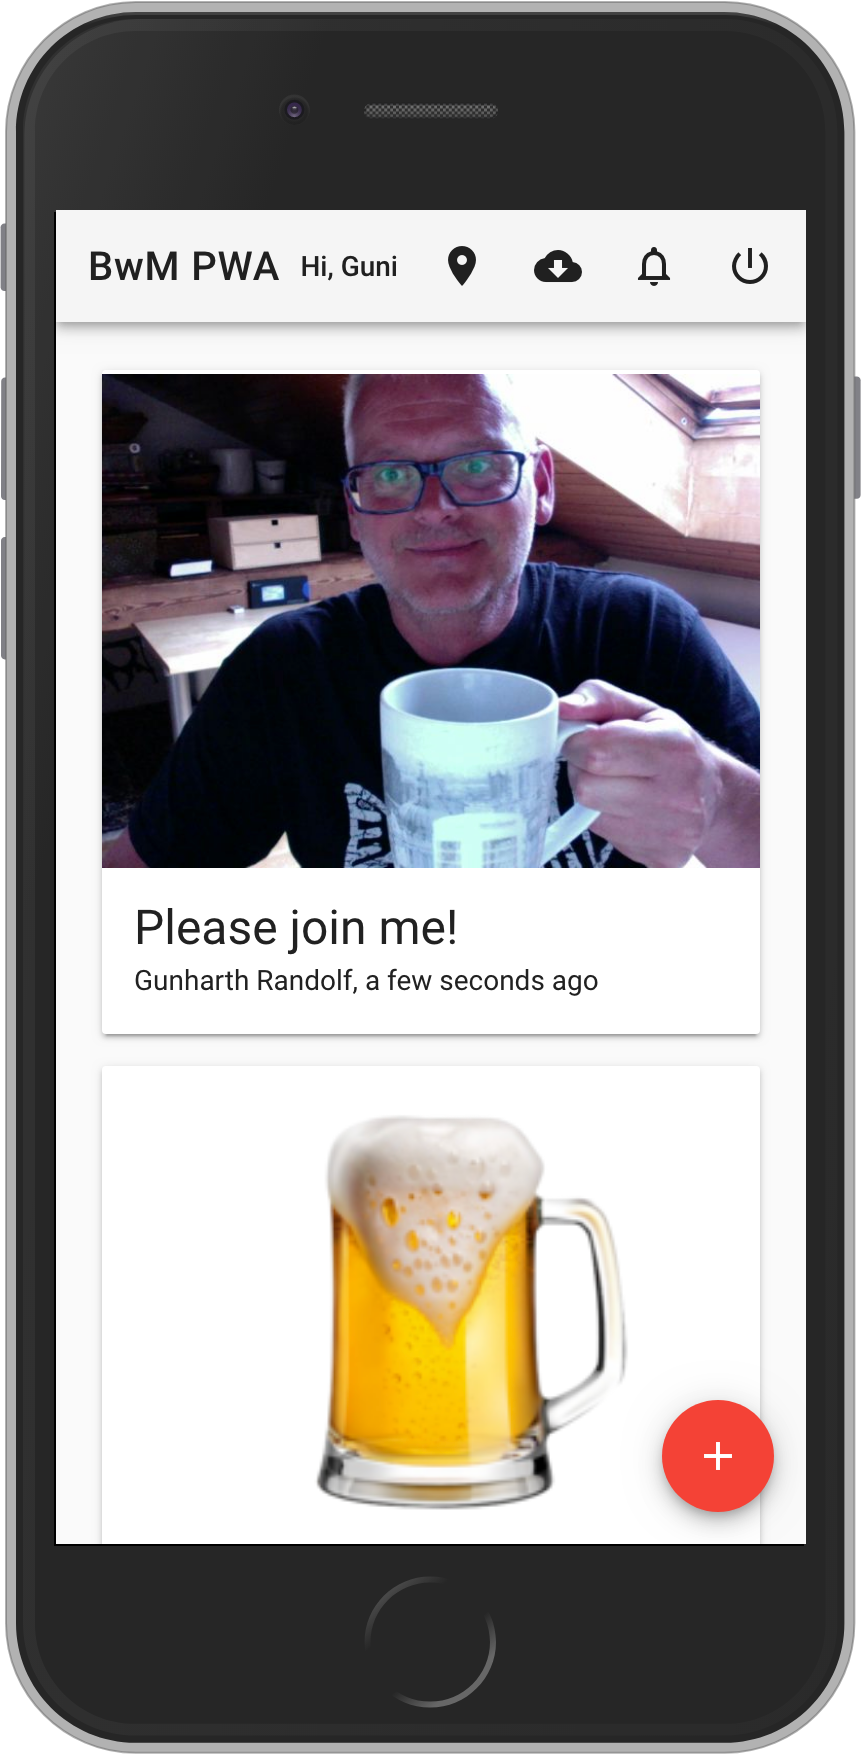
\includegraphics[width=.7\linewidth]{img/screen02}
    \caption{Main app screen}
    \label{fig:sub2}
  \end{subfigure}
  \begin{subfigure}{.5\textwidth}
    \centering
    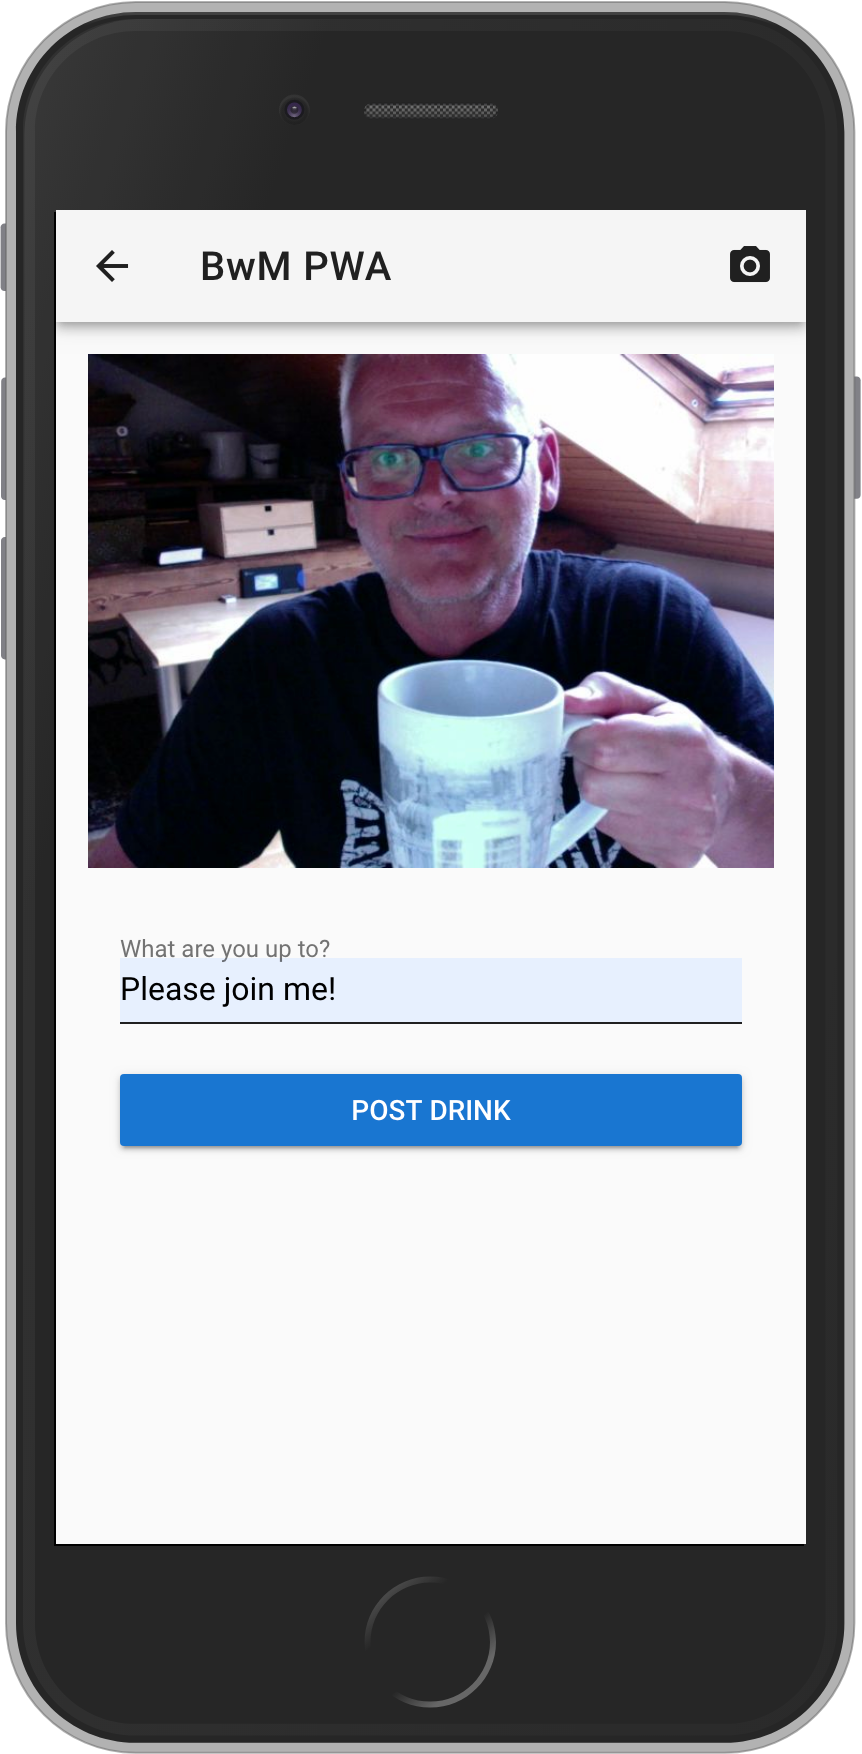
\includegraphics[width=.7\linewidth]{img/screen04}
    \caption{New post screen with photo option}
    \label{fig:sub1}
  \end{subfigure}%
  \begin{subfigure}{.5\textwidth}
    \centering
    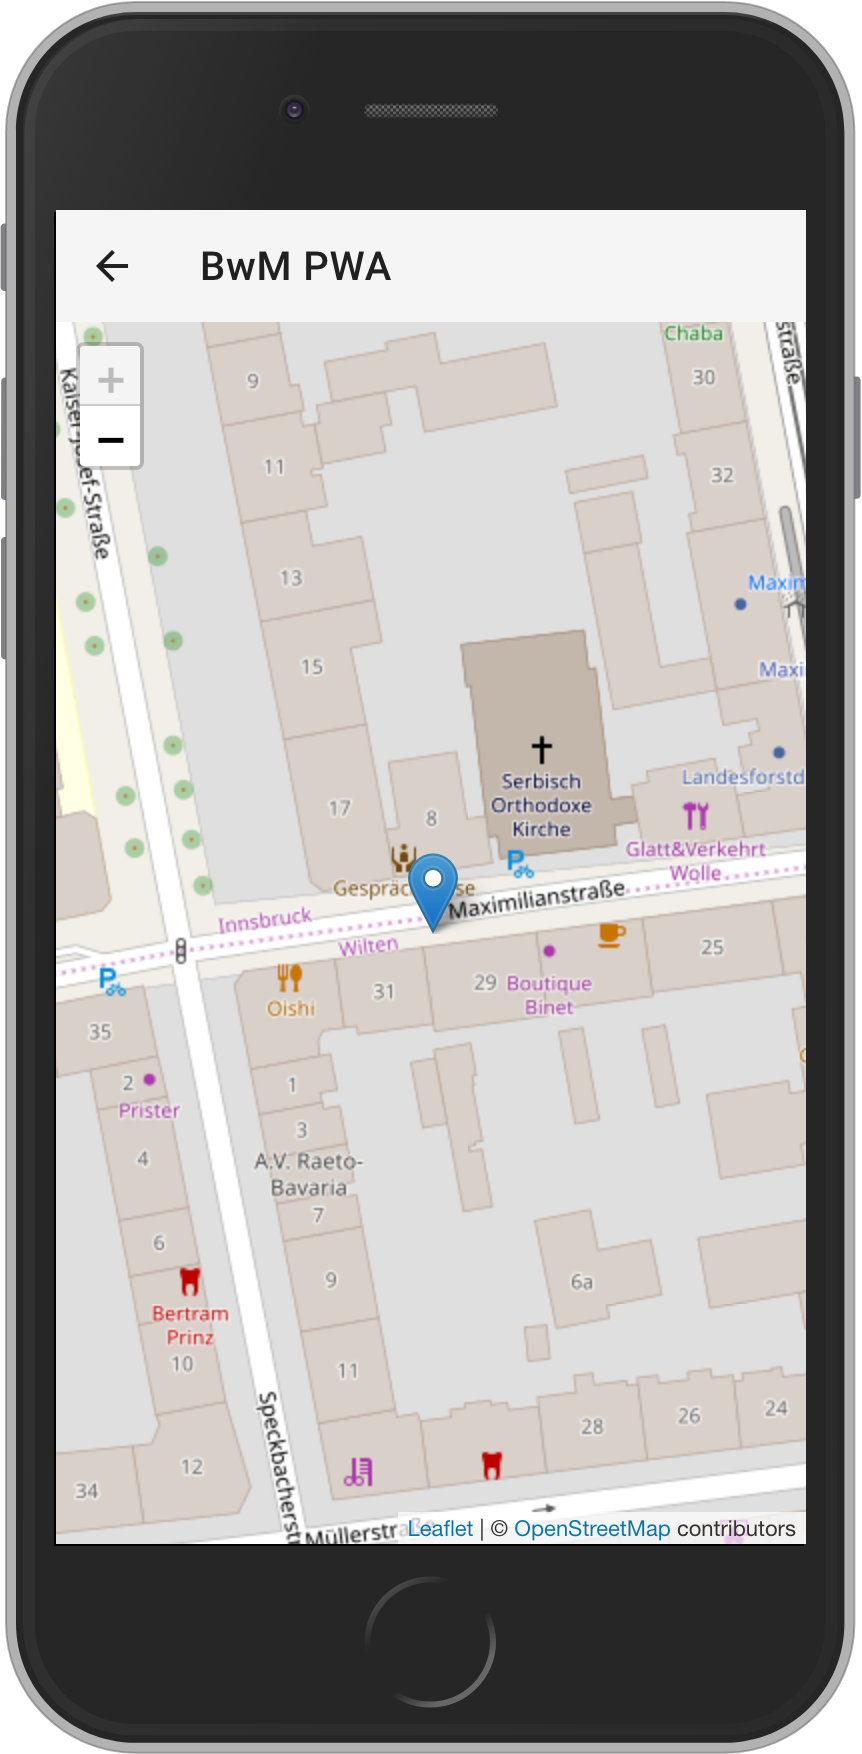
\includegraphics[width=.7\linewidth]{img/screen03}
    \caption{The map}
    \label{fig:sub2}
  \end{subfigure}
  \caption{Screenshots showing Vuetifys' material design components and the map}
  \label{fig:test}
\end{figure}
\pagebreak

Figure 3 shows the Lighthouse\footnote{\url{https://developers.google.com/web/tools/lighthouse}} Progressive Web App report for the \textit{Beer with Me} PWA.
\fig{img/lighthouse_test}{Lighthouse report}{fig:lighthouse}{1}


\subsection{Cloud Provider and Realtime Functionalities}

To cater for the back-end requirements I picked Firebase\footnote{\url{https://firebase.google.com}} as the provider. Around the same time in 2015, when the term Progressive Web Apps was born, Google acquired this San Francisco start-up. Since then Google has expanded upon the original service and integrated it closely into their other cloud ambitions - whereby the Firebase service is dedicated to providing a specialized Platform as a Service (PaaS) for mobile and web applications.

The following section demonstrates the Firebase services used for the \textit{Beer with Me} PWA.

To use Firebase in a project the following steps need to be performed:
\begin{enumerate}
  \item Register with Firebase
  \item Create a project
\end{enumerate}

\textbf{Authentication and Authorization}

Firebase Auth offers multiple methods to authenticate, including email and password and third-party providers like Google.

\begin{lstlisting}[language=JavaScript, caption=Firebase Auth initiation using VueJS (main.js), label=lst:firebase-auth]
  // Init Firebase auth before Vue inits the App
  firebase.auth.onAuthStateChanged(firebaseUser => {
    if (firebaseUser) {
      store.dispatch("autoSignIn", firebaseUser);
    }
    if (!app) {
      app = new Vue({
        router,
        store,
        render: h => h(App)
      }).$mount("#app");
    }
  });
\end{lstlisting}

\textbf{Realtime Database}
 feeding the feed of posts on the main application page. Map positions
JSON NoSQL

\begin{lstlisting}[language=JavaScript, caption=Realtime query for new posts (Home.vue), label=lst:firebase-listposts]
firebase.db
  .collection("drinks")
  .orderBy("created_at", "desc")
  .onSnapshot(snapShot => {
    this.drinks = [];
    snapShot.forEach(drink => {
      this.drinks.push({
        id: drink.id,
        url: drink.data().url,
        comment: drink.data().comment,
        author: drink.data().author,
        created_at: drink.data().created_at,
      });
    });
  });
\end{lstlisting}

\textbf{Realtime Push Notifications}

Firebase Functions

    \chapter{Results}

What answer was found to the research question; what did the study find? Was the tested hypothesis true?


Is it possible to take an existing mobile app and convert it to a PWA?

In summary,

What services and programming languages are a best fit in doing so?



How do those services and programming languages support the creation of a PWA?



What are the technical limitations, if any?

In conclusion, PWAs might not replace native apps completely within the next few years. However, the techniques involved have leveled up the standard of modern websites. Rapid enhancements of browser technologies promise further integration with devices and enduser behaviors.

One will have to wait and see when Apple and its Safari browser opens up. It may be assumed that with the pressure of Google


On the other hand, business wise? costs?


One a side note, it is puzzling that PWA as a technology has not yet arrived in the world of business and finance. Fact is, building and maintaining native mobile apps is expensive. Developing PWAs

    % \chapter{Discussion}

In conclusion, PWAs might not replace native apps completely within the next few years. However, the techniques involved have leveled up the standard of modern websites. Rapid enhancements of browser technologies and related standards promise further integration with browsers and devices.

The new Twitter website demonstrates that PWAs stepped out of the teething phase and are a serious contender for platform independent production ready applications. It is expected that this will entice other businesses to implement PWA technologies in the near future in order to streamline the delivery of their products.

A tighter integration for PWA development into existing frameworks, plugins and service providers will be necessary to raise the awareness for PWAs as a solid alternative to native and hybrid approaches.

Next too technical research on PWAs there is plenty of room for related future studies. The new technology introduces new user centric features in the likes of installing an app on a desktop PC, which implies studies on user behavior and usability. Further, PWAs have the potential to make app stores obsolete. The financial implications need to be researched and studies on possible future commercialization of PWAs are recommended.

    \chapter{Conclusion}

In conclusion, PWAs might not replace native apps completely within the next few years. However, the techniques involved have leveled up the standard of modern websites. Rapid enhancements of browser technologies and related standards promise further integration with browser and devices.

The new Twitter website demonstrates that PWAs stepped out of the teething phase and are a serious contender for platform independent production ready applications. We can expect further businesses to entice PWA technologies in the near future in order to streamline the delivery of their products.

Next too technical research on PWAs there is plenty of room for related future research. The new technology introduces new user behavior in the likes of installing a web site on a desktop PC, which implies research studies on user behavior and usability. Further, PWAs have the potential to make app stores obsolete. This financial aspect needs to be researched and a future outlook at new ways to commercialize PWAs is suggested.


    % This places the bibliography. You can add more
    % bibliographic items it the bibliography.bib file.
    % We suggest using a reference manager (e.g. Jabref)
    % to maintain this file
    \bibliography{bibliography}

    \newpage

    \begin{appendices}

        \backmatter

        % This is the actual appendix. The files referenced here
        % are just examples. You can add additional appendices
        % if necessary
        % \chapter{List of Interview Parners}

\Blindtext[2][6]

        % \chapter{Code Table}

\blindtext


    \end{appendices}

\end{document}
